% Niveau :      PCSI *
% Discipline :  Chimie Orga I
% Mots clés :   Spectrométrie UV-visible, Réactions acidobasiques

\begin{exercise}{Bleu de bromothymol}{2}{PCSI}
{Chimie organique I,Spectroscopie,UV-visible,Réactions acidobasiques}{bermu}

\begin{questions}
\questioncours Loi de Beer-Lambert. On fera bien attention de préciser les dépendances implicites des paramètres et les hypothèses de validité de la loi.

\begin{EnvUplevel}
    Le bleu de bromothymol (BBT) est un indicateur de pH très utilisé en biologie pour mettre en présence le $\mathrm{CO_2}$. Vers $\text{pH} = 7.0$, il passe de sa forme acide jaune à sa forme basique bleue (notées $\mathrm{InH}$ et $\mathrm{In^{-}}$) :\vspace{-1em}
    \begin{figure}[H]
        \centering
        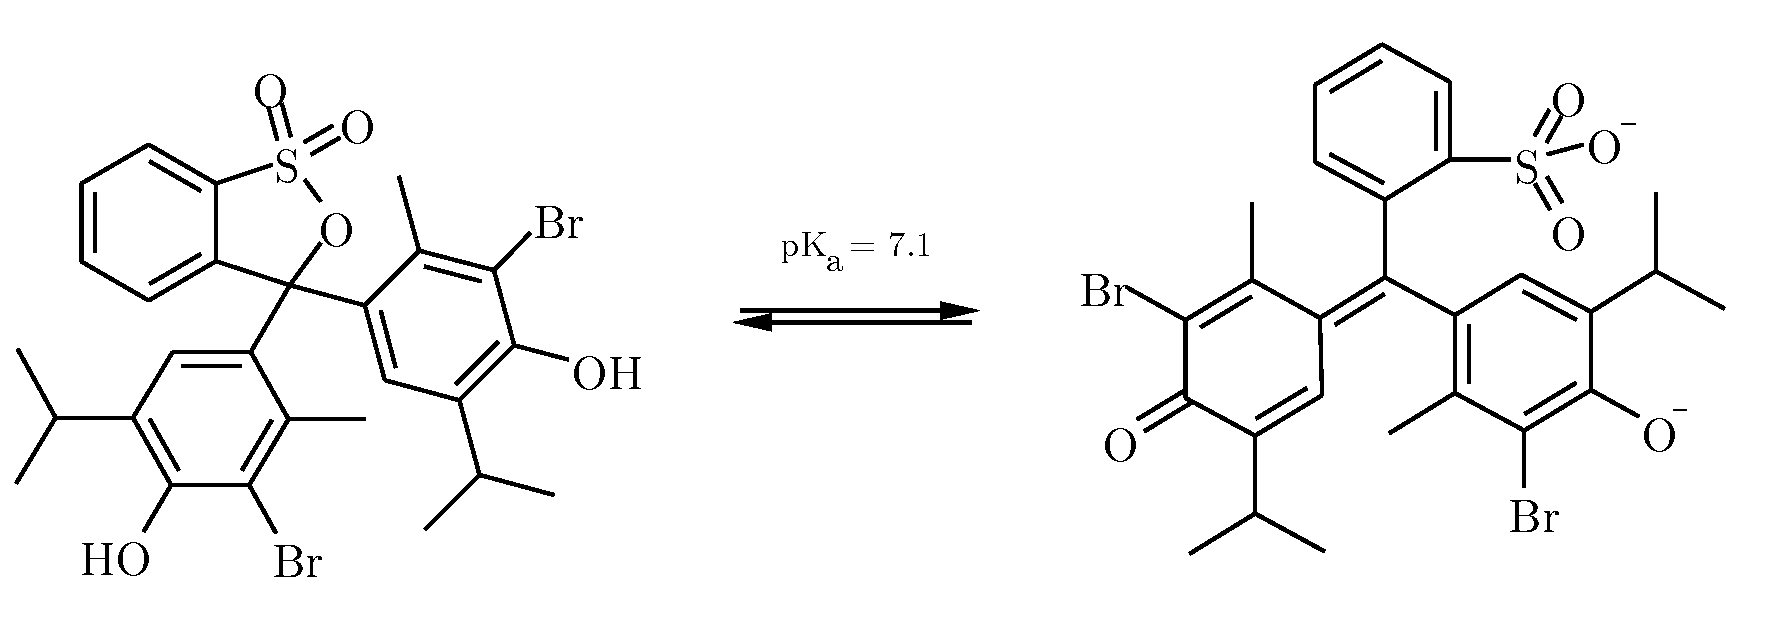
\includegraphics[width=.6\linewidth]{chimiePC/orga/BBT1.pdf}\vspace{-2em}
        \caption{\'Equilibre acidobasique du bleu de bromothymol.}
        \label{fig:BBT1}\vspace{-1em}
    \end{figure}
    
    Dans une publication récente (Hui Hou, \emph{Nature Scientific Reports}, 7:1759, 2017), les auteurs proposent une méthodologie pour mesurer le pH par mesure de l'absorbance.
    \begin{figure}[H]
        \centering
        \begin{tabularx}{\linewidth}{XX}
            \small{\textbf{(a)}} & \small{\textbf{(b)}}. \\
            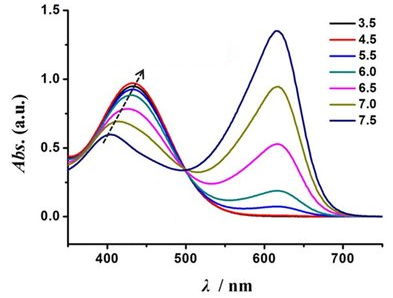
\includegraphics[width=\linewidth]{chimiePC/orga/BBT2.png} &
            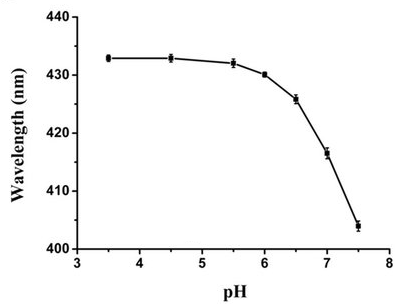
\includegraphics[width=\linewidth]{chimiePC/orga/BBT3.png}
        \end{tabularx}\vspace{-1em}
        \caption{Spectres d'absorption UV-Visible (\textbf{a}) et courbe de calibration du pic à $\sim$ 420 nm (\textbf{b}) du bleu de bromothymol pour différentes valeurs de pH.}
        \label{fig:BBT2}
    \end{figure}
\end{EnvUplevel}\vspace{-1em}

\question Interpréter qualitativement la fig. \ref{fig:BBT2}a avec les deux maxima $\lambda_\text{max,a} = 433$ nm et {$\lambda_\text{max,b} = 616$~nm}.

\question\label{qu:1} Rappeler l'intérêt de mesurer l'absorbance au niveau des maxima d'intensité et justifier que
$$A(\lambda) \simeq A_\text{max} + \dfrac{1}{2}\dv[2]{A}{\lambda} \qty(\lambda - \lambda_\text{max})^2 \qqtext{pour} \lambda \simeq \lambda_\text{max}.$$

\question Le point $\lambda_i = 500$ nm est nommé un point isobestique. Justifier par un simple calcul que ce point d'absorption constante $A_i$ durant la transformation $\mathrm{InH \xrightleftharpoons{} In^- + H^+}$ indique que cette transformation ne fait pas intervenir d'intermédiaire. \vspace{-2em}
\begin{EnvUplevel}
\paragraph{Indication :} exprimer l'absorbance de la solution en fonction des concentrations $[\mathrm{In^-}]$ et $[\mathrm{InH}]$.

On va maintenant s'intéresser à modéliser la courbe de calibration.
\end{EnvUplevel}

\question La forme basique du BBT possède également un maximum d'absorption en $\lambda_\text{max,b'} = 403$~nm. A l'aide de l'approximation de la question \ref{qu:1}, modéliser la longueur d'onde maximale $\lambda_\text{max}$ en fonction des concentrations $[\mathrm{In^-}]$ et $[\mathrm{InH}]$.
\end{questions}

\plusloin
\`A l'aide de la relation d'Henderson--Hasselbalch et du $\mathrm{pK_a}$ du BBT, exprimer la relation $\lambda(\text{pH})$. 
\end{exercise}